\chapter{Autoencoder}
The \textbf{autoencoder} are neural networks designed to learn efficient
representations of data, often for dimensionality reduction or feature extraction.
They are trained to attempt to copy its input to its output. This is achieved
with a network divided into two parts:
\begin{itemize}
    \item An \textbf{encoder} that maps the input to a hidden representation (latent space);
    \item A \textbf{decoder} that reconstructs the input from the hidden representation.
\end{itemize}

\begin{figure}[!ht]
    \centering
    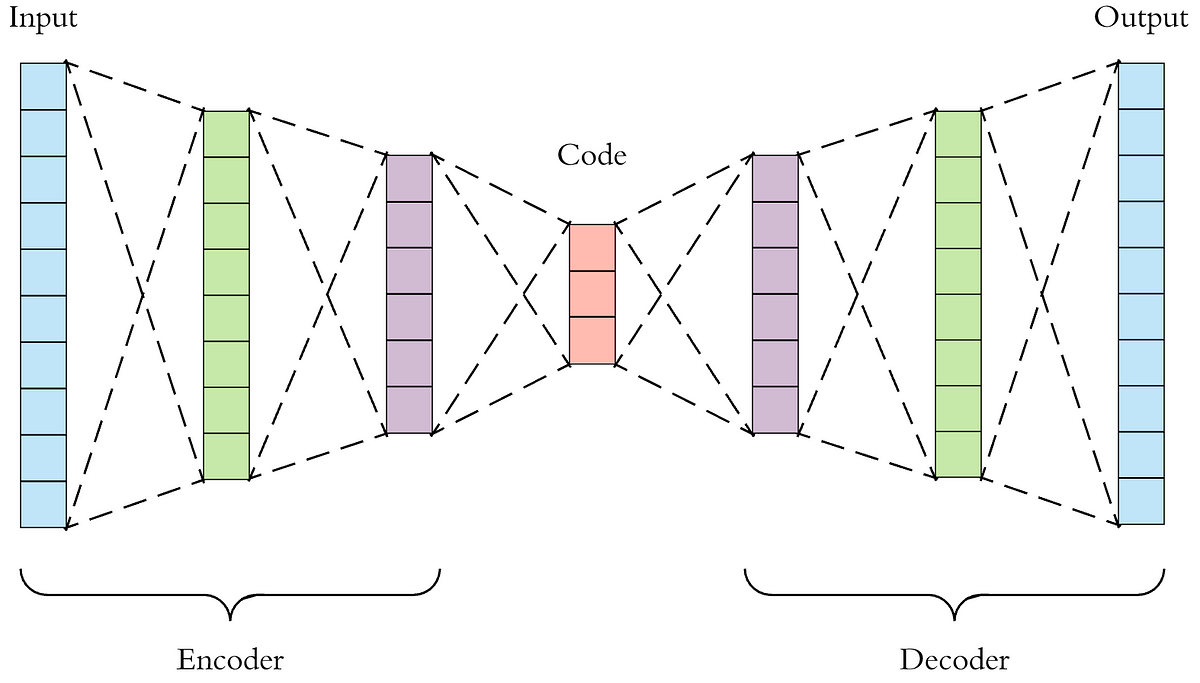
\includegraphics[width=0.7\textwidth]{img/Autoencoder/autoencoder.png}
    \caption{Autoencoder architecture}
    \label{fig:autoencoder}
\end{figure}

An autoencoder can be mathematically expressed as $h = f(x)$, where $h$ is the
latent representation of the input $x$. The output of the autoencoder is given by
$\hat{x} = g(h) = g(f(x))$, where $g$ is the decoder function. The autoencoder is
trained to minimize the reconstruction error, i.e., the difference between the
input $x$ and its reconstructed output $\hat{x}$, aiming for $\hat{x} \approx x$.

This structure forces the model to select which aspects of the data to preserve,
thereby learning potentially useful properties of the data.
\section{Types of Autoencoder}
\subsection{Undercomplete Autoencoder}
An \textbf{undercomplete autoencoder} has a latent space (hidden layer) that is
smaller in dimensionality than the input. This design forces the autoencoder to
compress the input, encouraging it to capture the most significant features of
the data.

This model is trained to minimize the reconstruction error, i.e. the difference
between the input and the output. The loss function is usually the \textit{mean
    squared error} (MSE) between the input and the output.
\begin{equation}
    \mathcal{L}(x, g(f(x))) = ||x - g(f(x))||^2
\end{equation}
\begin{note}
    If the activation functions in the encoder and decoder are linear, an 
    undercomplete autoencoder is equivalent to Principal Component Analysis (PCA).
\end{note}

We could have non linear autoencoder, where the encoder and decoder are non-linear
functions. This allows the autoencoder to learn more complex representations of
the data.
\subsection{Regularized Autoencoder}
\textbf{Regularized autoencoder} are autoencoder that are trained to minimize the
reconstruction error, but also have a regularization term. This term is used to
prevent the autoencoder from learning the identity function.

Regularized autoencoders can be further categorized as follows:
\begin{itemize}
    \item \textbf{Sparse autoencoder}: is a regularized autoencoder where the
          hidden layer is greater than the input layer. Usually we add a
          regularization term to the loss function to penalize the activation
          of the hidden units. This type must respond to statistical features of
          the dataset, rather than acting as an identity function.
    \item \textbf{Denoising autoencoder}: are basic autoencoder where the task
          is to reconstruct the input without noise. The input is corrupted by
          adding some noise, and the autoencoder is trained to reconstruct the
          original input.
    \item \textbf{Stacked autoencoder}: are autoencoder where the encoder and
          decoder are composed of multiple layers. This allows the autoencoder
          to learn more complex representations of the data.
    \item \textbf{Variational Autoencoder}: are autoencoder that are trained to
          learn the parameters of the probability distribution that generates
          the data. This allows the autoencoder to generate new data similar to
          the training data. The middle layer of the autoencoder is used to
          represent the mean and the variance of the distribution. And, the loss
          function need to be improved to take into account the difference between
          the probability distribution of the input and the output.
          \begin{figure}[!ht]
                \centering
                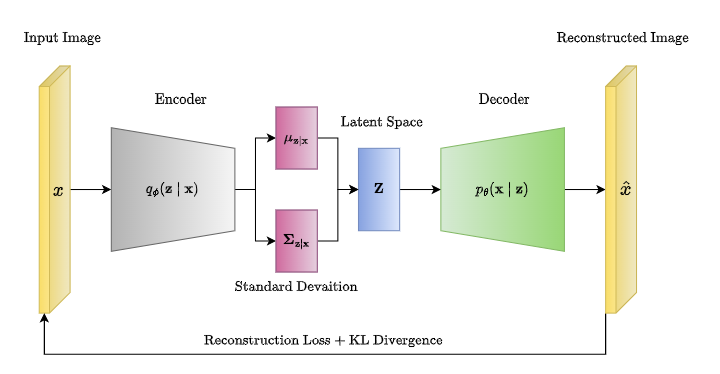
\includegraphics[width=0.7\textwidth]{img/Autoencoder/VAE.png}
                \caption{Variational Autoencoder architecture}
                \label{fig:variational_autoencoder}
          \end{figure}
\end{itemize}